\subsubsection{Scénario Cockburn}
\textbf{Cas d'utilisation:} Payer le passage

\textbf{Acteur primaire:} Conducteur

\textbf{Acteur support:} Le poste de surveillance et opérateur humain (si le borne est manuelle)

\textbf{Pré-condition: }  la borne est opérationnelle

\textbf{Post-condition: }  la transaction(paiement) est acceptée.

\textbf{Scenario primaire: } \\ 
    \textbf{1.} Le conducteur paye en liquide %(\ref{subsec:paieLiquide}) 
    \\ 
    \textbf{2.} La transaction est enregistrée dans l’ordinateur central de la société d’autoroute.\\ 

\textbf{Variantes:}\\
    \textbf{1a.} Le conduteur paye par carte
    \\
    \textbf{1b.} Le conducteur paye par télépéage.
     \\
    \textbf{1d.} la transaction(paiement) a échoué. Retourne à l’état 1. \\ %he clicks in the botton who calls the technicien 
\newpage
\subsubsection{Décomposition de cas d'utilisation (Généralisation):} 
\begin{figure}[h]
    \centering
    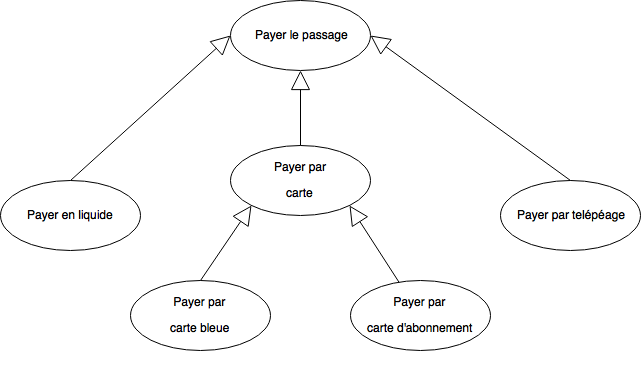
\includegraphics[scale=0.5]{02_Desenvolvimento/TD2/images/PayeGeneralisation.png}
    \caption{Généralisation de cas d'utilisation: Payer le passage}
\end{figure}
\subsubsection{Collaboration}
\begin{figure}[h]
    \centering
    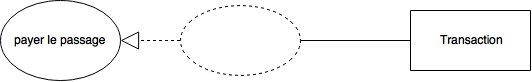
\includegraphics[scale=0.6]{02_Desenvolvimento/TD2/images/ColaPayer.png}
    \caption{Diagramme d'activité: Payer le passage}
\end{figure}
\newpage
\subsubsection{Diagramme d'activité}
\begin{figure}[h]
    \centering
    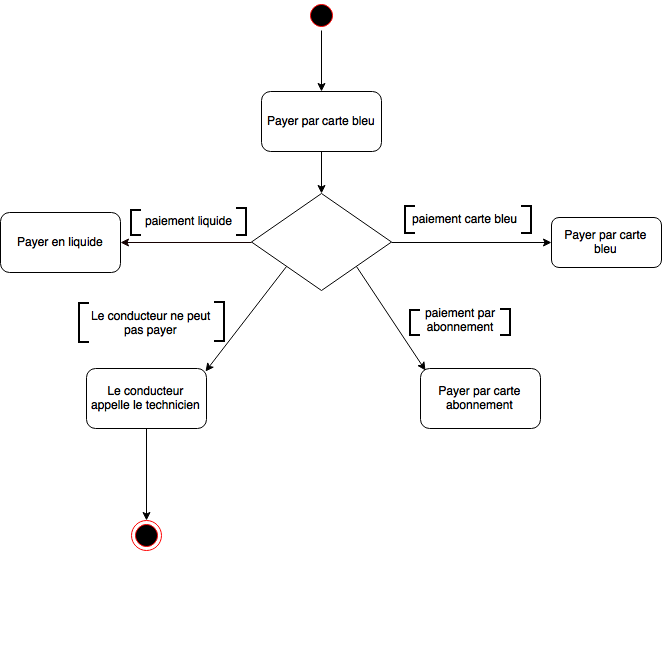
\includegraphics[scale=0.6]{02_Desenvolvimento/TD2/images/DAPayePassage.png}
    \caption{Diagramme d'activité: Payer le passage}
\end{figure}
